\chapter{Design}
\label{sec:design}

% Ist das zentrale Kapitel der Arbeit. Hier werden das Ziel sowie die
% eigenen Ideen, Wertungen, Entwurfsentscheidungen vorgebracht. Es kann
% sich lohnen, verschiedene Möglichkeiten durchzuspielen und dann
% explizit zu begründen, warum man sich für eine bestimmte entschieden
% hat. Dieses Kapitel sollte - zumindest in Stichworten - schon bei den
% ersten Festlegungen eines Entwurfs skizziert werden.
% Es wird sich aber in einer normal verlaufenden
% Arbeit dauernd etwas daran ändern. Das Kapitel darf nicht zu
% detailliert werden, sonst langweilt sich der Leser. Es ist sehr
% wichtig, das richtige Abstraktionsniveau zu finden. Beim Verfassen
% sollte man auf die Wiederverwendbarkeit des Textes achten.

% Plant man eine Veröffentlichung aus der Arbeit zu machen, können von
% diesem Kapitel Teile genommen werden. Das Kapitel wird in der Regel
% wohl mindestens 8 Seiten haben, mehr als 20 können ein Hinweis darauf
% sein, daß das Abstraktionsniveau verfehlt wurde.

%%%%%%%%%%%%%%%%%%%%%%%%%%%%%%%%%%%%%%%%%%%%%%%%%%%%%%%%%%%%%%%%%%%%%%%%%%%%%%%%
%                                                                              %
% MOTIVATION                                                                   %
%                                                                              %
%%%%%%%%%%%%%%%%%%%%%%%%%%%%%%%%%%%%%%%%%%%%%%%%%%%%%%%%%%%%%%%%%%%%%%%%%%%%%%%%
% Checked
\section{Motivation}
\label{sec:motivation}

These days, complex simulation applications no longer fit on a single
computing device like a desktop computer. Therefore, parallel
computers are necessary instruments in scientific computing where time
to solution is important and a large amount of memory is required.  To
exploit the performance of a parallel computer, the application need
to be distributed onto the computing environment and exchange data by
communication over a network.

Assume, the mentioned parallel computer is a compute cluster
(Section~\ref{sec:cluster}). Furthermore assume, that cluster nodes
are equal among each other (\emph{vertical homogeneous}) and a node
provides only one type of computing hardware (\emph{horizontal
  homogeneous}). Usually, simulation applications are prepared for
this kind of vertical and horizontal heterogeneous clusters by domain
decomposition (Section~\ref{sec:domain_decomposition}). The simulation
domain is decomposed by a fixed algorithm into smaller chunks of work
called \emph{subdomains} and mapped onto the homogeneous network of
nodes. Subdomains exchange simulation specific data through predefined
paths among each other. This could mean in concrete terms of MPI
(Section~\ref{sec:mpi}), that every MPI process manages a subdomain and
communicates with a fixed set of other MPI processes by fixed
communication operations. The simulation algorithm and the
decomposition method defines what, when and with whom a process
communicates.  Figure~\ref{fig:state_of_the_art} shows this for a
one-to-one mapping from a domain onto a cluster.

\begin{figure}[H]
  \centering 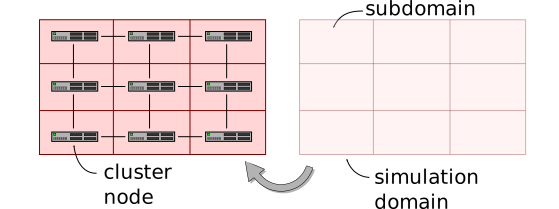
\includegraphics[width=\textwidth]{graphics/30_state_of_the_art}
  \caption{State of the art: the simulation domain is decomposed in
    subdomains. Subdomains are mapped one-to-one onto the homogeneous
    compute cluster.}
  \label{fig:state_of_the_art}
\end{figure}

For most simulations computed on cluster systems is this approach
state of the art.  This approach works, as long as both hardware and
simulation stay in this fixed relationship. Thus, there is no change
necessary as long as a simulation will always be executed on the same
cluster, with the same network topology, and the same algorithms
describing the simulation model.

However, it is not possible to map all modern simulations in this
model of a homogeneous world, some simulation applications have also
vertical and horizontal heterogeneous behavior.  In vertical
direction, multiscale effects, each representing a specific algorithm
of the simulation, lead to varying communication topologies between
subdomains. Every communication topology usually requires
sophisticated programming, that can be quite time consuming.  In
horizontal direction, the workload of subdomains vary throughout the
time of simulation. Therefore, sooner or later the simulation runs
into an unbalanced state of workload distribution. That unbalanced
state do neither saturates all available computing resources nor does it
reduce overall simulation time to its minimum. Furthermore, a globally
increased workload might require a redistribution of the simulation
domain onto the computing nodes.

Not only the simulation can be heterogeneous, but also the cluster
hardware on which the simulation is executed
(Section~\ref{sec:accel}): vertical cluster heterogeneity is the
development of cluster nodes to multisocket, multicore and
additional accelerator hardware, where each of these compute devices
has its own hierarchical memory structure. This hardware needs to be
programmed with caution and knowledge about the device to achieve
maximal performance.  Also, horizontal differences of cluster nodes
are possible. For example, a cluster can consist of varying node
types for different tasks in the simulation application. Therefore,
the simulation domain can not be mapped one-to-one on such a cluster
configuration, but rather the mapping should be configurable
explicitly. Figure~\ref{fig:heterogeneous_cluster_node} shows such
an explicit mapping from the simulation domain onto a heterogeneous
computing system. This example computing systems shows several device
hierarchies. A single node has two sockets each equipped with a
multicore CPU and each CPU has access to a pair of accelerator
devices.

\begin{figure}[H]
  \centering
  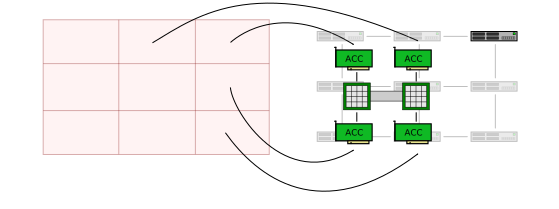
\includegraphics[width=\textwidth]{graphics/30_heterogeneous_cluster_node}
  \caption{Explicit mapping of subdomains onto the computing nodes of
    a heterogeneous and hierarchical computing system}
  \label{fig:heterogeneous_cluster_node}
\end{figure}

A real world example for such heterogeneous behavior of simulations is
the PIConGPU simulation (Section \ref{sec:picongpu}). While magnetic
and electric fields only influence their directly neighboring fields,
which requires next neighbor communication, particles interact
globally with each other, which requires an all-to-all communication
algorithm.  Furthermore, during the time of the simulation, particles
can move to other subdomains, which leads to an unbalanced
distribution of particles over the entire simulation domain. On the
hardware side, PIConGPU is developed for the execution on cluster
systems with NVIDIA accelerator hardware.  CPUs are responsible for
data offloading and communication over the network, some of the
available accelerators compute the interaction of fields and
particles, while others generate a visualization of the simulated
data. Thus, vertical and horizontal heterogeneity both in simulation
domains and on the hardware cluster are already present in real world
simulation applications.

Nowadays, state of the art communication libraries can not be adapted
to the needs of modern simulation applications.  Therefore, there
should be an interlayer between simulation application and the
software stack of the cluster. This layer should allow for an explicit
mapping of the simulation domain onto the communication library, while
the communication library should be easily exchangeable. With such a
setup, the mapping can be adjusted to heterogeneous behavior of
simulation application and cluster hardware.  As an added benefit,
this layer can be used to address problems like load balancing and
fault tolerance. However, both of these problems will not be addressed
by this system directly. Instead it should be possible to build an
application that supports both fault tolerance and load balancing
based on this system.

To address these issues, an approach for a flexible mapping of
communication processes onto arbitrary communication libraries was
designed This design will be presented in the following
sections. First of all, the requirements for such a system are
discussed. It is followed by a description of the overall design and
finally the design of each component is discussed in detail.
%%%%%%%%%%%%%%%%%%%%%%%%%%%%%%%%%%%%%%%%%%%%%%%%%%%%%%%%%%%%%%%%%%%%%%%%%%%%%%%%
%                                                                              %
% ANALYSIS OF PIConGPU CODE                                                    %
%                                                                              %
%%%%%%%%%%%%%%%%%%%%%%%%%%%%%%%%%%%%%%%%%%%%%%%%%%%%%%%%%%%%%%%%%%%%%%%%%%%%%%%%
%% \section{Analyzing the PIConGPU Application}
%% \label{sec:picongpu_analysis}

%% The analysis of the PIConGPU source code and modeled simulation domain
%% plays as significant role in the design of the developed system.

%% The PIConGPU domain is divided into a three-dimensional grid of cells.
%% Each cells computes effects of particles and fields. Fields interact
%% with fields of neighboring cells. Therefore, is a communication with
%% neighboring cells necessary. Particles interact with all other
%% particles. Therefore, is a all-to-all communication with all other
%% cells necessary.

%% PIConGPU uses plain MPI as communication back end. Some MPI calls
%% are covered by a communicator class, some are used directly in
%% the source code. Data exchange of neighboring cells is performed
%% by non-blocking point-to-point operations. Certain algorithms
%% make use of collective operations to collect data among a particular
%% amount of cells.


%%%%%%%%%%%%%%%%%%%%%%%%%%%%%%%%%%%%%%%%%%%%%%%%%%%%%%%%%%%%%%%%%%%%%%%%%%%%%%%%
%                                                                              %
% REQUIREMENTS                                                                 %
%                                                                              %
%%%%%%%%%%%%%%%%%%%%%%%%%%%%%%%%%%%%%%%%%%%%%%%%%%%%%%%%%%%%%%%%%%%%%%%%%%%%%%%%
% Checked
\section{Requirements}
\label{sec:requirements}

The previous Section~\ref{sec:motivation} described the state of the
art of simulations on cluster systems and gave a motivation to solve
the problems of modern simulations.
%% Furthermore, analyzed
%% Section~\ref{sec:picongpu_analysis} the PIConGPU application with
%% respect to its needs for a enhanced communication approach.
It was
claimed that an interlayer between application and communication
library is required.  This interlayer should offer the possibility to
describe the communication processes of the simulation in a very
general manner.  The construction of this interlayer involves three
steps.  First of all, existing communication libraries should be
abstracted by a general communication interface. Thus, communication
is not restrict to a single communication library and, therefore,
makes the simulation more portable.  Furthermore, the communication
topology of the simulation should be modeled explicitly.  So that, the
modeled communication topology can be mapped explicitly onto an
communication abstraction layer.  Finally the combination of modeled
communication topology and the abstraction from communication
libraries form an approach to communicate virtually on basis of the
described communication topology.  In summary, the discussion on the
interlayer result in the following four requirements of the referred
problems of modern simulations:

\begin{enumerate}
\item Abstract data exchange method
\item Description of the communication topology
\item Mapping of communiation topology onto the abstract topology
\item Virtual data exchange method 
\end{enumerate}



%%%%%%%%%%%%%%%%%%%%%%%%%%%%%%%%%%%%%%%%%%%%%%%%%%%%%%%%%%%%%%%%%%%%%%%%%%%%%%%%
%                                                                              %
% THE SYSTEM                                                                   %
%                                                                              %
%%%%%%%%%%%%%%%%%%%%%%%%%%%%%%%%%%%%%%%%%%%%%%%%%%%%%%%%%%%%%%%%%%%%%%%%%%%%%%%%
% Checked 
\section{Design of the System}

Physical networks such as Ethernet, Infiniband or Myrinet are the
foundation of communication libraries such as MPI
(Section~\ref{sec:mpi}).  State of the art simulation applications are
usually implemented directly on these existing communication
libraries. The developed system introduces an interlayer between
application and communication library (Figure \ref{fig:design}). This
layer fulfills all requirements set up in
Section~\ref{sec:requirements}. Figure \ref{fig:design} shows the
individual components of the interlayer and which requirement they
fulfill. The communication abstraction layer, on top of the existing
communication library, abstracts the communication interface.  A graph
is used to model the communication topology of the simulation domain
and a graph-based virtual overlay network maps this graph onto the
hardware topology of the communication abstraction layer.

\begin{figure}[H]
  \centering 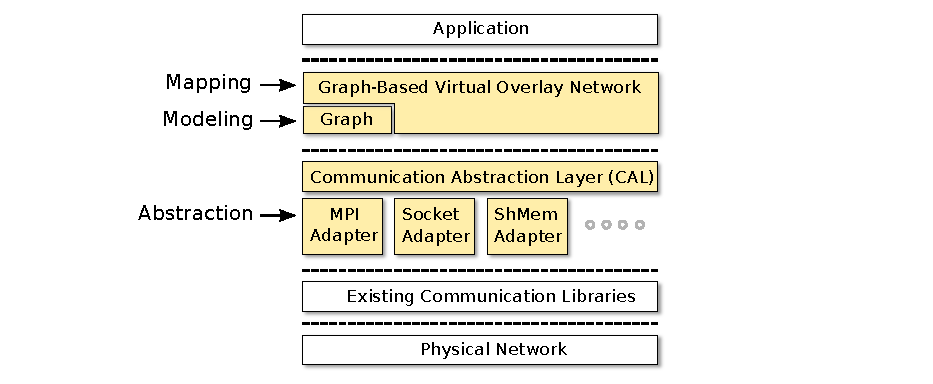
\includegraphics[width=\textwidth]{graphics/30_design}
  \caption{Design of the developed system in layers. An intermediate
  layer between application and communication library is introduced.}
  \label{fig:design}
\end{figure}

This section presents the design of the system that fulfills the
previously discussed requirements (Section~\ref{sec:requirements}).
It will discuss each component in detail, starting with the
communication abstraction layer in
Section~\ref{sec:comm_abstraction}. The graph interface is
described in Section~\ref{sec:graph}, finally, the graph-based virtual
overlay network is introduced in Section~\ref{sec:gvon}. Component
interfaces will be described in some cases by pseudo-code which is
strongly related to the C++ programming language. It is assumed, that
the reader has a basic knowledge of programming and function
interfaces.

%%%%%%%%%%%%%%%%%%%%%%%%%%%%%%%%%%%%%%%%%%%%%%%%%%%%%%%%%%%%%%%%%%%%%%%%%%%%%%%%
%                                                                              %
% COMMUNICATION ABSTRACTION LAYER                                              %
%                                                                              %
%%%%%%%%%%%%%%%%%%%%%%%%%%%%%%%%%%%%%%%%%%%%%%%%%%%%%%%%%%%%%%%%%%%%%%%%%%%%%%%%
% Checked
\section{Abstraction from Existing Communication Libraries}
\label{sec:comm_abstraction}

% Motivation for communication abstraction
Simulation applications can be interconnected by a vast variety of
communication libraries. Most simulations utilize exactly one possible
libarary, but this restricts the simulation to computing systems which
only support the selected library (Figure
\ref{fig:design_state_of_the_art}).

\begin{figure}[H]
  \centering 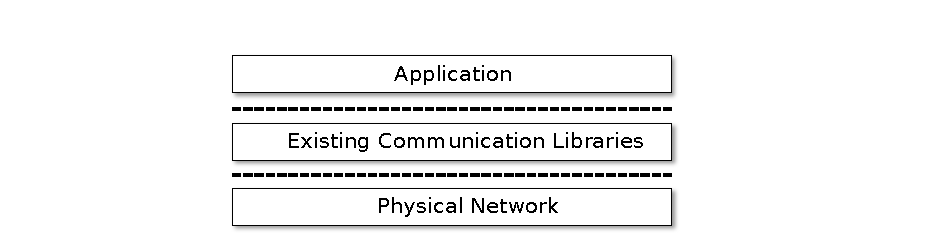
\includegraphics[width=\textwidth]{graphics/30_design_state_of_the_art}
  \caption{State of the art: simulation applications are implemented directly
  on top of the communication library.}
  \label{fig:design_state_of_the_art}
\end{figure}

Assuming that a simulation, distributed on a several computers, uses a
communication library based on TCP/IP sockets. The execution of this
simulation on a single machine is an interesting use case for
testing. It results in no problem when the simulation is executed on
this local machine and communicates locally by sockets.  But, it might
be more efficient to use shared memory to exchange data between
subdomains, instead of TCP/IP messages.

However, replacing one interface for data exchange by another requires
usually a lot of reprogramming of the communication logic. Therefore,
it is not a sufficient solution for the problem.  Rather, varying
communication libraries should by addressable by the same
communication interface to make the application portable for varying
computing environments. Although, there are existing standards for
communication in cluster systems, the world of computer science is
subject to constant change.  The possibility to exchange the
underlying layer without changing the interface to this layer is a
precondition for future applications in distributed computing.  Thus,
the abstraction from this existing communication libraries is a
fundamental property for a portable application.

The challenge is to provide a very general interface, that provides
the possibility to address varying communication libraries through it.
This interface should be as common as possible and should be easily
deployable into existing applications by replacing the actual
communication library without changing the fundamental understanding
of the way to communicate within this application. The following
section describes the design of such an abstract communication
interface.


%%%%%%%%%%%%%%%%%%%%%%%%%%%%%%%%%%%%%%%%%%%%%%%%%%%%%%%%%%%%%%%%%%%%%%%%%%%%%%%%
%                                                                              %
% CAL                                                                          %
%                                                                              %
%%%%%%%%%%%%%%%%%%%%%%%%%%%%%%%%%%%%%%%%%%%%%%%%%%%%%%%%%%%%%%%%%%%%%%%%%%%%%%%%
% Checked
\subsection{Communication Abstraction Layer (CAL)}
\label{sec:cal}

The \textit{Communication Abstraction Layer}, short \textit{CAL}, is a
general communication interface on top of an existing communication
library. The libraries are accessible through adapters, which makes it
possible to access varying communication libraries. By exchanging the
adapter, the application based on the interface can be ported to
varying communication libraries without changing interface function
calls. The CAL is configured with a certain adapter at compile
time. Thus, by using this flexible approach, no run-time overhead
should occur.

While the CAL provides an abstract interface for common communication
methods, needs the adapter to implements the interface demanded by the CAL.
Particular communication operations are performed by existing
communication libraries encapsulated in an adapter.

Instances participating on communication in general are subsequently
called peers.  The interface of the CAL provides basic point-to-point
communication operations (Section~\ref{sec:des:p2p}), collective
operations (Section~\ref{sec:cal_collective}) and operations for
grouping of peers (Section~\ref{sec:cal_context}).  Figure
\ref{fig:cal} shows the communication abstraction layer on top of
existing communication libraries.  The CAL with a specific adapter
could already replace a certain communication library in a simulation
application, but it is not meant to be the level of abstraction the
simulation programmer will interact with. The design of further layers
of abstraction will be discussed in Sections \ref{sec:graph} and
\ref{sec:gvon}.

\begin{figure}[H]
  \centering
  
\includegraphics[width=\textwidth]{graphics/30_design_cal}
  \caption{Communication Abstraction Layer (CAL) on top of existing
    communication layers. Varying communication libraries can be
    addressed through the CAL interface, when an according adapter for
    this library is implemented.}
  \label{fig:cal}
\end{figure}


Using the CAL instead of a concrete communication library has
the advantage, that only the adapter needs to be replaced when
changing the communication environment, for example when migrating
to another compute architecture. Although, the application has
to be recompiled, the CAL interface stays the same.


%The CAL has the requirement, that peers need to be connected directly
%by the network of the adapter.
%Peers have to be connected directly by the network of the
%adapter.
%Because, It is not planed that the CAL provides routing
%abilities.
%No routing makes it impossible to forward data between
%different adapters of the CAL. Thus a specific CAL only provides a
%single adapter.
%But several CALs can be used with different adapters
%to communicate on several networks.
%In such a scenario a kind of
%routing can be implemented on top of the CAL by the system
%user.
%Therefore, the design was first pushed forward in the direction
%of a single adapter design and considerations regard to a multiple
%adapter design is left open for future work.


%%%%%%%%%%%%%%%%%%%%%%%%%%%%%%%%%%%%%%%%%%%%%%%%%%%%%%%%%%%%%%%%%%%%%%%%%%%%%%%%
%                                                                              %
% ADDRESSING OF PEERS                                                          %
%                                                                              %
%%%%%%%%%%%%%%%%%%%%%%%%%%%%%%%%%%%%%%%%%%%%%%%%%%%%%%%%%%%%%%%%%%%%%%%%%%%%%%%%
% Checked
\subsection{Addressing of Peers}
% CAL virtual addressing
Each communication library provides a particular approach to address
peers, which can be quiet different. Internet socket based systems
address their peers by IP addresses, MPI based systems address their
processes by ranks and shared memory based systems are utilizing
memory addresses.  These diverse approaches to address peers in a
network need to be translated to an unified address space to provide a
singular interface for the CAL user.  Therefore, the CAL provides a
virtual address, short \emph{vAddr}, which is an unique identifier for
its peer. The Based on this virtual address, peers are able to address
each other through the CAL interface.

The translation of virtual addresses to the adapter specific real
address is resolved by the adapter itself. Thus, the adapter defines
how the participants of its network are mapped onto the given virtual
address space of the CAL. This mapping is hidden from the CAL, so that
the CAL only needs to handle virtual addresses and the adapter handles
its particular address space.

%%%%%%%%%%%%%%%%%%%%%%%%%%%%%%%%%%%%%%%%%%%%%%%%%%%%%%%%%%%%%%%%%%%%%%%%%%%%%%%%
%                                                                              %
% CAL INTERFACE                                                                %
%                                                                              %
%%%%%%%%%%%%%%%%%%%%%%%%%%%%%%%%%%%%%%%%%%%%%%%%%%%%%%%%%%%%%%%%%%%%%%%%%%%%%%%%
% Peer2Peer Operations
\subsection{Point-to-Point Communication Methods}
\label{sec:des:p2p}

In the first place provides the CAL point-to-point communication
methods. These are basic communication methods to exchange abitrary
data between two peers, such as sending and receiving data.  These
methods are available blocking and non-blocking variants.

A Non-blocking communication method returns an \emph{Event} object that represents
the state of the only just executed communication method. The state
of the event is either \emph{ready} or \emph{not ready}. An
event provides a function to request the current state and a function
to  wait until the method has finished. The CAL only provides the
event interface. Adapters implement the  event interface for their
particular communication library since each libary treats non-blocking
communication differently \cite{ref:mpi_specification,ref:boost_asio}.

A point-to-point communication method is called with a triplet of
arguments, including the virtual address of sender or receiver, the
message description tag and the actual data object to exchange.  The
interface is influenced by existing communication libraries that all
share a common interface \cite{ref:boost_mpi, ref:boost_asio,
  ref:zmq}. The message description tag is a simple header of the
message. It helps to easily distinguish between messages of the same
sending peer.  The data object should provide methods to retrieve the
data pointer and the size of the data. The data pointer should point
to a contiguous memory area. The following list shows the
point-to-point communication methods of the CAL interface:

\begin{itemize}
  %% \item  \textbf{void send(destinationVAddr, tag, data);}
  %% \item  \textbf{void recv(sourceVAddr, tag, data);}
  %% \item  \textbf{Event asyncSend(destinationVAddr, tag, data);}
  %% \item  \textbf{Event asyncSecv(sourceVAddr, tag, data);}

  \item  void \textbf{send }( destinationVAddr, tag, data);
  \item  void \textbf{recv }( sourceVAddr, tag, data);
  \item  Event \textbf{asyncSend }( destinationVAddr, tag, data);
  \item  Event \textbf{asyncSecv }( sourceVAddr, tag, data);

\end{itemize}

%%%%%%%%%%%%%%%%%%%%%%%%%%%%%%%%%%%%%%%%%%%%%%%%%%%%%%%%%%%%%%%%%%%%%%%%%%%%%%%%
%                                                                              %
% CONTEXT                                                                      %
%                                                                              %
%%%%%%%%%%%%%%%%%%%%%%%%%%%%%%%%%%%%%%%%%%%%%%%%%%%%%%%%%%%%%%%%%%%%%%%%%%%%%%%%
% Checked
\subsection{Grouping of peers}
\label{sec:cal_context}
Grouping of peers is, next to the communication methods, the most
important function the CAL provides through its interface.  By
default, all peers of the CAL are grouped to a global group of peers.
A group of peers will be called \textit{context}. Therefore, the
global group of peers is called global context. A context is valid for
all contained peers. In turn, it is invalid for all peers not
contained.

A context stores the set of virtual addresses of its contained peers , the
number of peers grouped, and whether the context is valid for a particular
peer. It is the base for communication algorithms with more than 2
participating peers.
% These algorithm are introduced as collective operations (Section \ref{sec:cal_collective}).

The CAL provides always the global context from which a peer can
retrieve its global virtual address. A new context can be created from
a subset of peers of an already existing context. Thus, a new context
can be created according to the requirements of the communication
algorithm. This new context provides its own virtual address space,
thus, the virtual address of a peer is context dependent.

Each adapter can handle contexts differently. The CAL only
defines the context interface, but each adapter needs to implement the
context interface for its particular communication
library. The adapter must respect that a virtual address
is context dependent. Therefore, the mapping of a virtual address to a
real address has to be adapted to the currently used context.

%%%%%%%%%%%%%%%%%%%%%%%%%%%%%%%%%%%%%%%%%%%%%%%%%%%%%%%%%%%%%%%%%%%%%%%%%%%%%%%%
%                                                                              %
% COLLECTIVE OPERATIONS                                                        %
%                                                                              %
%%%%%%%%%%%%%%%%%%%%%%%%%%%%%%%%%%%%%%%%%%%%%%%%%%%%%%%%%%%%%%%%%%%%%%%%%%%%%%%%
% Checked
\subsection{Collective Operations}
\label{sec:cal_collective}
A \textit{collective operation}, short \textit{collective}, is a
communication pattern that is executed simultaneously by all peers of
a context. For example are collectives utilized to collect, distribute,
share and reduce data.  Each collective can be implemented by a
sequence of peer to peer operations, but communication libraries,
especially the ones for high performance calculations such as MPI
(Section~\ref{sec:mpi}), often provide optimized collective support.

A collective is always executed with respect to a context and the
result is either received by a single peer, the root, or by all peers.
While a large number of collectives is known to the parallel
computation commmunity, the CAL only provides the most common ones
with respect to the analysis of the PIConGPU source code
(Section~\ref{sec:picongpu}).  However, Other collectives are easily
deploy able in future work. The following is a list of all provided
collective operations of the CAL and their description:


\begin{itemize}
\item  void \textbf{gather} (rootVAddr, context, send, recv)\\
  Collection of data elements from every peer in the context. Each peer
  contributes the same number of data elements. The collected data will
  be received from the root peer.

\item void \textbf{allGather} (context, send, recv)\\
  Similar to gather(), but all peers of the context receive the data.

\item  void \textbf{scatter} (rootVAddr, context, send, recv)\\
  Distribution of data elements from the root peer to all other peers of
  the context. The data will be divided into chunks of same
  size. Assuming the number of data elements is divisible by the number
  of peers, every peer will receive the same number of data
  elements. Thus, every peer receives different data elements.

\item  void \textbf{allScatter} ( context, send, recv)

  Similar to scatter(), but all peers of the context receive the same.

\item  void \textbf{reduce} (root, context, binOperation, send, recv)\\
  Reduction of the data elements from every peer of a context
  by a binary function that takes arguments of an arbitrary type
  and returns a values of the same type.

\item  void \textbf{allReduce}  (context, operation, send, recv)\\
  Similar to reduce(), but all peers of the context receive the
  result of the reduction.

\item  void \textbf{broadcast} (root, context, data)\\
  Distributes data elements from the root peer to all other peers of
  the context. Every peer receives the same data elements.

\item  void \textbf{syncronize} (context)\\
  This operation synchronizes the control flow of all peers of the
  context.

\item  void \textbf{createContext} (peers, context)\\ 
  Creation of a new context from a subset of peers of an already
  present context.

\end{itemize}

\noindent All peers of the listed collectives send or receive the same number of
elements.  But some algorithms require an exchange of varying number
of elements. Therefore, collectives like gather, allGather, scatter,
allScatter are also available in a variant with varying number of
elements per peer. These collectives get an additional receive count
argument, that describes how many data elements each peer has
contributed to the collective.


%%%%%%%%%%%%%%%%%%%%%%%%%%%%%%%%%%%%%%%%%%%%%%%%%%%%%%%%%%%%%%%%%%%%%%%%%%%%%%%%
%                                                                              %
% GRAPH                                                                        %
%                                                                              %
%%%%%%%%%%%%%%%%%%%%%%%%%%%%%%%%%%%%%%%%%%%%%%%%%%%%%%%%%%%%%%%%%%%%%%%%%%%%%%%%
% Checked
\section{Modeling of the Application Domain by a Graph}
\label{sec:graph}
A simulation model is usually implemented through a particular
algorithm in the simulation application.  Porting this algorithm onto
a parallel computing system requires a decomposition
(Section~\ref{sec:domain_decomposition}) of the simulation domain into
a set of subdomains.  Assume, subdomains need to interact among each
other, communication between subdomains is necessary. Thus, the
algorithm determines the communication topology of the simulation.

\todo{Refer to requirement}

%% Communication topologies are often implemented in a implicit and
%% static fashion. A change of the simulation algorithm needs to be translated
%% into a change of the corresponding communication patterns, which can
%% be quiet costly. Furthermore, would a reutilization of already modeled
%% communication topologies reduce implementation effort of
%% implementations of future simulations.

%% \paragraph*{}
%% A more elegant approach is the explicit modeling of relationships
%% between the subdomains. Therefore, the communication topology of the
%% simulation.

The most general method to model a topology is a
\emph{graph}~\cite{ref:graph}. Furthermore, has the explicit modeling
of the communication topology by a graph the advantage that the reuse
of this topology reduces implementation effort of future simulation
applications.  From a mathematical perspective, a graph is a pair of
vertices and edges. Edges are pairs of vertices. So to speak, a graph
represents a set of objects, where some of these objects are connected
by links.

% directed cycle multi graph
Vertices of the graph used in further descriptions are connected by
directed edges.  Loops and multiple edges between two vertices are
allowed (Figure~\ref{fig:graph}). The resulting graph is a directed
multigraph with loops. The mathematical expression for this kind of
graph is quiver \cite{ref:quiver}.

\begin{figure}[H]
  \centering 
\includegraphics[width=\textwidth]{graphics/30_graph}
  \caption{The graph interface describes quivers. It is shown a
    directed cycle multi graph with four vertices. Graphs can be
    used to describe the communication topology of domain decomposed
    applications.}
  \label{fig:graph}
\end{figure}

\noindent Changing the simulation algorithm implies a different
communication topology and in turn implies a different graph. The
graph has the advantage, that the communication topology is
modeled explicitly. It is not necessary to rewrite the simulation
application as long as the application is based on the topology
information provided by the graph. Thus, communication processes can
by implemented on top of the graph description. The presented graph
should be addressable by the following interface:

\begin{itemize}
  \item VertexList \textbf{getVertices} ()\\
    Returns the list of all vertices of the graph.
    
  \item  Vertex \textbf{getVertex} (index)\\
    Returns a particular vertex by vertex \textit{index}.

  \item  VertexList \textbf{getAdjacentVertices} (vertex)\\
    Returns a list of all adjacent vertices of \textit{vertex}.

  \item  EdgeList \textbf{getOutEdges} (vertex)\\
    Returns a list of all outgoing edges from the \textit{vertex}
    paired with their target vertex.

  \item  EdgeList \textbf{getInEdges} (vertex)\\
    Return a list of all incoming edges to the \textit{vertex}
    paired with their source vertex.

  \item  Graph \textbf{createSubGraph} (vertices)\\
    Returns a subgraph, that only contains the defined
    \textit{vertices} from the supergraph.
\end{itemize}

%%%%%%%%%%%%%%%%%%%%%%%%%%%%%%%%%%%%%%%%%%%%%%%%%%%%%%%%%%%%%%%%%%%%%%%%%%%%%%%%
%                                                                              %
% GRAPH PROPERTIES                                                             %
%                                                                              %
%%%%%%%%%%%%%%%%%%%%%%%%%%%%%%%%%%%%%%%%%%%%%%%%%%%%%%%%%%%%%%%%%%%%%%%%%%%%%%%%
% Checked
\subsection{Properties}
A graph viewed in isolation is only a representation of connected
vertices, not providing further information. Interpreting the graph as
a container offers the possibility to insert objects into the graphs
vertices and edges.

An object that resides in this containers will be called property and
is introduced as a concept to annotate a graph. A property usually
provides subdomain information and can be bound to vertices and edges
(Figure \ref{fig:property}). Each vertex and edge of the same graph
share respectively the same type of property. A graph annotated with
properties is significantly more meaningful and therefore helps to
keep the connection of the simulation domain and communication
topology.

\begin{figure}[H]
  \centering 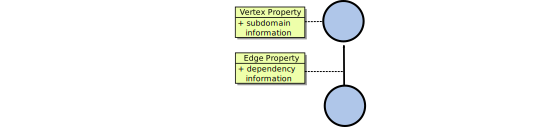
\includegraphics[width=\textwidth]{graphics/30_property}
  \caption{A graph annotated with both vertex and edge property. The vertex
    property primarily describe a subdomain. The edge property
    describe the dependencies between subdomains.}
  \label{fig:property}
\end{figure}

\noindent The field of application of properties can by diverse. It highly
depends on the graph and its area of utilization.  A Property can also
be used to create a connection between a pair of graphs, providing a
hierarchical description.



%%%%%%%%%%%%%%%%%%%%%%%%%%%%%%%%%%%%%%%%%%%%%%%%%%%%%%%%%%%%%%%%%%%%%%%%%%%%%%%%
%                                                                              %
% MODELING GAME OF LIFE AS A GRAPH                                             %
%                                                                              %
%%%%%%%%%%%%%%%%%%%%%%%%%%%%%%%%%%%%%%%%%%%%%%%%%%%%%%%%%%%%%%%%%%%%%%%%%%%%%%%%
% Checked
\subsection{Modeling Game of Life as a Graph}
\label{sec:gol}
To give an example for modeling a specific simulation application,
Figure~\ref{fig:gol_modeling} shows the modeling of the Game of Life
(GoL)~\cite{ref:gol} domain by a graph. GoL simulates the evolution of
a set of cells for an abitrary amount of time steps. The cells are
arranged in a two-dimensional grid (Figure \ref{fig:gol_simulation}).
A cell has a state which is either alive or not alive and the state of
the next time step is calculated by rules.  The common set of rules
determine the state of a cell for the next time step by the current
state information of the neighboring cells.  Assume the rule: a dead
cell with exactly 3 living cells in the neighborhood will be reborn on
the next time step is the only existing rule in further descriptions
of GoL.  Nevertheless, a GoL simulation can consist of a arbitrary set
of rules.

\begin{figure}[H]
  \centering 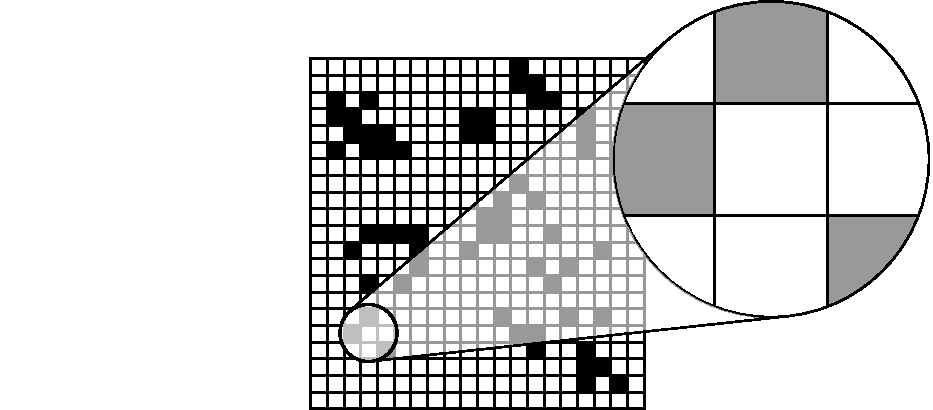
\includegraphics[width=\textwidth]{graphics/30_gol_simulation}
  \caption{A GoL domain with a cut out of 9 neighboring cells. The GoL
    domain is a rectangular grid of cells.  Cells have a state, while
    living cells are colored dark, dead cells are white. The state of
    a cell for the next time step is determined by a set of rules.}
  \label{fig:gol_simulation}
\end{figure}

\noindent The GoL simulation providing only a single rule is modeled as follows:
every cell is represented by a vertex and neighboring cells are
connected by an edge.  Each vertex has the property \emph{cell}, which
contains the state of the cell. Figure \ref{fig:gol_modeling} shows a
vizualized cut out of the modeled GoL domain. To determine the next
state of a cell, it has to count the living adjacent cells. The cell
will be alive on the next time step, if exactly three adjacent cells
are alive.


\begin{figure}[H]
  \centering 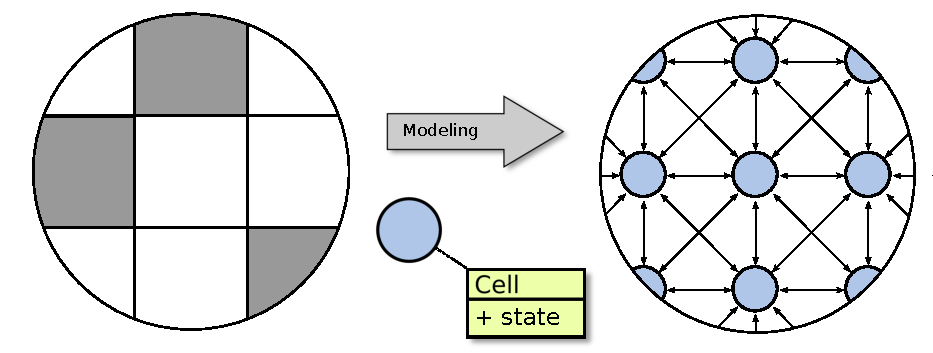
\includegraphics[width=\textwidth]{graphics/30_gol_modeling}
  \caption{Cut-out of a Game of Life domain (on the left) was modeled
    as a graph (on the right). Each Vertex is described by the vertex
    property cell, containing the state information of the cell. A
    Vertex determines its next state by the state of neighboring
    cells.}
  \label{fig:gol_modeling}
\end{figure}

\noindent The rule is now changed slightly: a cell is alive on the next time
step when at least one diagonal neighbor is alive.  A changed rule
 implies a change in the GoL algorithm.  This changes the GoL
communication topology and therefore the modeled
graph. Figure~\ref{fig:gol_modeling_changed} models the GoL domain
with the changed rule. Vertices are connected with its diagonal
located vertices. Nevertheless, to determine the next state of a cell
the number of living adjacent cells have to be counted.

\begin{figure}[H]
  \centering 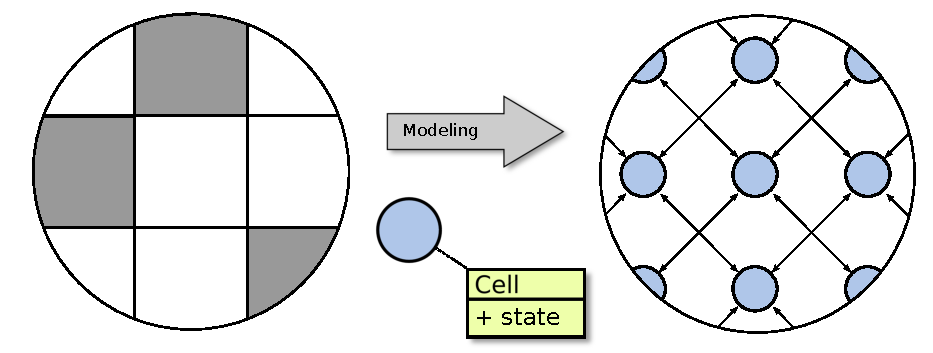
\includegraphics[width=\textwidth]{graphics/30_gol_modeling_changed}
  \caption{Cut-out of a Game of Life domain (on the left) modeled
    with a different rule. Only diagonal located vertices are connected.
  A Vertex still determines its next state by state of neighboring cells}
  \label{fig:gol_modeling_changed}
\end{figure}


%%%%%%%%%%%%%%%%%%%%%%%%%%%%%%%%%%%%%%%%%%%%%%%%%%%%%%%%%%%%%%%%%%%%%%%%%%%%%%%%
%                                                                              %
% PARTITIONING THE GoL GRAPH                                                   %
%                                                                              %
%%%%%%%%%%%%%%%%%%%%%%%%%%%%%%%%%%%%%%%%%%%%%%%%%%%%%%%%%%%%%%%%%%%%%%%%%%%%%%%%
% Checked
\subsection{Partitioning the GoL Graph}
The graph in Figure~\ref{fig:gol_modeling} models the GoL domain very fine
granular by every individual cell. While it is the smallest possible
domain decomposition, it might not be very efficient when a single cell
is calculated by a single process. A process can computer
considerably more cells.

Figure~\ref{fig:gol_bundle} shows the creation of a partitioned graph
by bundling multiple vertices. A parition of vertices is called a
bundle. These Bundles are connected by edges when at least one cell on
the border of a bundle is the neighbor cell of a border cell from
another bundle.  The creation of a partioned graph by bundles with a
minimum of connections is the topic of graph partitioning algorithms.

While the fine granular GoL graph represents the GoL cells in detail,
the partitioned graph represents dependencies of bundled cells.GoL
graph and partitioned graph can coexist and be connected by its
properties Thus, the properties of the partioned graph changed with
respect to the GoL graph, so that, bundles store the bundled cells and
the bundle connections refer to cells in neighboring bundles.

\begin{figure}[H]
  \centering 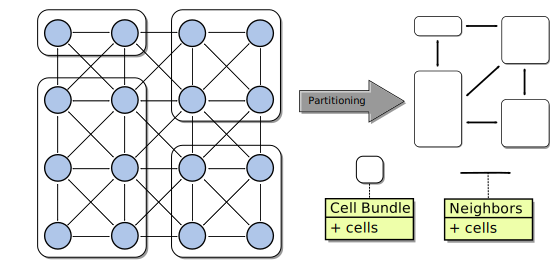
\includegraphics[width=\textwidth]{graphics/30_gol_bundle}
  \caption{The GoL graph is partitioned by bundling multiple
    cells. The properties of the partioned graph have changed with
    respect to the GoL graph. The vertex property contains the cells
    of a bundle, while the edge property contains information about
    border cells in neighboring bundles.}
  \label{fig:gol_bundle}
\end{figure}

The partitioned graph could be used as foundation to distribute GoL to
multiple nodes of a cluster. Each bundle could be calculated by its own
process. The processes calculate a time step of their local GoL graph and
communicate the states of their border cells to adjacent bundles.

It has been introduced a different approach to model the Game of Life
domain. It were used the same description language, the graph.  Fine
granular modeled domains can be partioned by common graph partition
algorithm to obtain possibly more performance by clustering
vertices. A automated transformation from a graph description into a
more efficient graph description is an interesting topic, but not
covered by this work.


%%%%%%%%%%%%%%%%%%%%%%%%%%%%%%%%%%%%%%%%%%%%%%%%%%%%%%%%%%%%%%%%%%%%%%%%%%%%%%%%
%                                                                              %
% MODELING GAME OF LIFE AS A GRAPH                                             %
%                                                                              %
%%%%%%%%%%%%%%%%%%%%%%%%%%%%%%%%%%%%%%%%%%%%%%%%%%%%%%%%%%%%%%%%%%%%%%%%%%%%%%%%
% Checked
\subsection{Modeling a N-Body Simulation as a Graph}
\label{sec:design:nbody}
%% The second example to model a simulation application by a graph should provide
%% a completely different algorithm in respect to GoL. 

%% The N-body simulation, with a totally different algorithm in respect to GoL, was chosen as the
%% second example to model a simulation application by a graph.

The N-body simulation simulates particles in an two or three
dimensional space influenced by physical forces. The force considered
for this simulation is the gravity among each particle.  A particle is
described by its mass $m$, location $\overrightarrow{r}$ and velocity
$\overrightarrow{v}$.  The gravitational force between two particles
$i$ and $j$ can be calculated in a two-body model with the
gravitationlal constant $G$ by the Equation~\ref{eq:two_body_force}:

\begin{equation}
  \label{eq:two_body_force}
  \overrightarrow{F_{i,j}} = G  m_i  m_j \cdot \frac{\overrightarrow{r_j} - \overrightarrow{r_i}}{|\overrightarrow{r_j} - \overrightarrow{r_i}|^3}
\end{equation}

\noindent Equation~\ref{eq:n_body_force} describes the gravitational force of
particle $i$ to all other N-1 particles as the sum of each particular
force $\overrightarrow{F_{i,j}}$.

\begin{equation}
  \label{eq:n_body_force}
  \overrightarrow{F_{i,n}} = \sum_{j = 0 \atop j \neq i}^{N-1} \overrightarrow{F_{i,j}}
\end{equation}

\noindent Therefore, the force affecting particle $i$ is calculated by
considering velocity, mass and location of all other
particles. Modeling the dependencies, resulting from the simulations
algorithm, results in an all-to-all communication pattern with a
complexity of $o(N^2)$. Figure~\ref{fig:nbody_modeling} models the
N-body domain with $N = 6$ as a fully connected graph. Particles are
represented as pentagon in a two-dimensional space. The size of the
particles signals its mass and the arrow its velocity and direction.
In the modeling, a vertex represents a particle and all particles are
connected by an edge. A vertex has the property particle that includes
the particle mass, location and velocity.

\todo{Borders of grid are ugly}
\begin{figure}[H]
  \centering 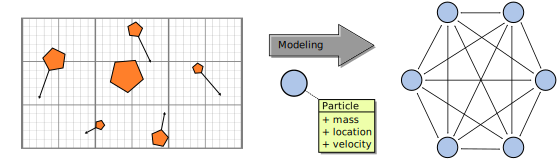
\includegraphics[width=\textwidth]{graphics/30_nbody_modeling}
  \caption{Modeling of an N-body domain with $N = 6$. A particle is
    represented by a vertex and each vertex is connected to all other
    vertices by edges.}
  \label{fig:nbody_modeling}
\end{figure}

\noindent A gravitational force on the particle $i$ results in a change of its velocity and
location after a fixed amount of time $t$. The following equations describe these
changes.

\begin{align}
  \label{eq:n_body_update}
  \overrightarrow{a} =&~ \frac{\overrightarrow{F_{i,n}}}{m}\\
  \overrightarrow{v} =&~ \overrightarrow{a} \cdot t + \overrightarrow{v_0}\\
  \overrightarrow{r} =&~ \frac{\overrightarrow{a}}{2} \cdot t^2 + \overrightarrow{v_0} \cdot t + \overrightarrow{r_0}
\end{align}


%%%%%%%%%%%%%%%%%%%%%%%%%%%%%%%%%%%%%%%%%%%%%%%%%%%%%%%%%%%%%%%%%%%%%%%%%%%%%%%%
%                                                                              %
% GRAPH-BASED VIRTUAL OVERLAY NETWORK (GVON)                                   %
%                                                                              %
%%%%%%%%%%%%%%%%%%%%%%%%%%%%%%%%%%%%%%%%%%%%%%%%%%%%%%%%%%%%%%%%%%%%%%%%%%%%%%%%
% Checked
\section{Graph-Based Virtual Overlay Network (GVON)}
\label{sec:gvon}
The previous sections described the tools to communicate in between
peers and to model a communication topology. The combination of these
tools establish a virtual communication layer within the simulation
domain. This layer is created by an explicit mapping of the
communication topology onto the abstract communication
layer. Therefore, an application domain and its according
communication topology modeled by a graph can be used to perform
communication processes between subdomains.  This section introduces a
\textit{graph-based virtual overlay network}, short \textit{GVON},
that is based on the graphs and the CAL.

The graph does provide a simulation domain specific communication
topology.  It is used as a blueprint for the virtual network topology.
Communication operations are provided by the CAL as base for the
overlay network.  Figure \ref{fig:gvon} shows the GVON as a layer
between the graph and CAL on one side and the application on the other
side.

\begin{figure}[H]
  \centering 
\includegraphics[width=\textwidth]{graphics/30_gvon}
  \caption{The graph-based virtual overlay network provides
    communication functionality based on the CAL, but uses the
    communication topology modeled by a graph.}
  \label{fig:gvon}
\end{figure}

\noindent All peers that want to take part on the communication of the GVON need
to know exactly the same graph. In order to ensure that, the graph can be
constructed in parallel by all peers, loaded from the same file of a
distributed file system or could even be delivered by a master
peer. Furthermore, peers need to use the same adapter configuring its
CAL, otherwise a communication is not possible.


%%%%%%%%%%%%%%%%%%%%%%%%%%%%%%%%%%%%%%%%%%%%%%%%%%%%%%%%%%%%%%%%%%%%%%%%%%%%%%%%
%                                                                              %
% GVON MAPPING                                                                 %
%                                                                              %
%%%%%%%%%%%%%%%%%%%%%%%%%%%%%%%%%%%%%%%%%%%%%%%%%%%%%%%%%%%%%%%%%%%%%%%%%%%%%%%%
% Checked
\subsection{Mapping of a Graph to the CAL}
\label{sec:mapping}
The connection between a graph and the CAL is a mapping of vertices
to peers, called the \emph{vertex map}.  A vertex map is valid for a
certain graph. Furthermore, the GVON provides a mapping of  graphs
to contexts (Section~\ref{sec:cal_context}), called the \emph{graph
  map}. This mapping is necessary since the GVON will also be used to
map collective operations on a graph to the CAL.  The vertex and
graph map are the basis for the mapping of communication processes
to the communication abstraction layer.  The mapping of vertices to
peers and graphs to contexts is a joint process of all peers that want
participate in the communication based on a particular graph.This
mapping process is divided into two phases.

\subsubsection*{First Phase: Distribute}
The first phase distributes vertices of a graph to the peers, whereby
every vertex is assigned to a peer.  Figure~\ref{fig:gvon_mapping}
shows 3 peers and a graph of 4 vertices that are mapped to the
peers. It is possible that more than one vertex is mapped to a peer.
There are a varity of methods to distribute the vertices.  It could be
done totally randomized, round robin, consecutive, or even dictated by
some master peer. The distribution behavior is defined by the user of
the GVON and might be object for further optimization.

\begin{figure}[H]
  \centering 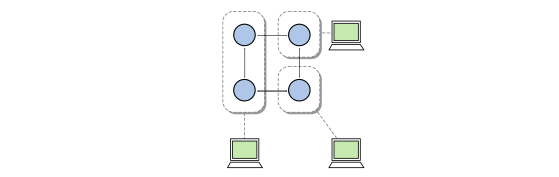
\includegraphics[width=\textwidth]{graphics/30_gvon_mapping}
  \caption{All vertices of a graph are distributed onto 3 peers. The
    vertices are not distributed evenly, thus, one peer is host for 2
    vertices.}
  \label{fig:gvon_mapping}
\end{figure}

\subsubsection*{Second Phase: Announce}
In the second phase, the peers announce their mapped vertices to all
other peers.  A peer that announces vertices is called host and the
announced vertices are called hosted vertices.  Every host receives
from every other host a list of its hosted vertices.  This list is
used to update the vertex map and to create a new context only
including the hosts. The new context will be bounded to the graph of
the hosted vertices in the graph map.  A host is responsible for the
communication of its hosted vertices.  So to speak, it is also
possible that a host is responsible for all vertices of a graph and
communicates finally always with itself.  Depending on the used
adapter this might not even be a problem, since communication of a
peer with itself can be performed in shared memory and does not
necessarily include network latency.


%%%%%%%%%%%%%%%%%%%%%%%%%%%%%%%%%%%%%%%%%%%%%%%%%%%%%%%%%%%%%%%%%%%%%%%%%%%%%%%%
%                                                                              %
% GVON COMMUNICATION                                                           %
%                                                                              %
%%%%%%%%%%%%%%%%%%%%%%%%%%%%%%%%%%%%%%%%%%%%%%%%%%%%%%%%%%%%%%%%%%%%%%%%%%%%%%%%
% Checked
\subsection{Communication within the GVON}
From the perspective of an overlay network, a vertex is interpreted as
a virtual peer, edges between adjacent vertices indicate that the
virtual peers are able to communicate with each other. An application,
implemented on top of the GVON, has the transparent view of exchanging
messages between vertices. The GVON is taking care, that the messages
reach the correct vertex host.  Finally, this is the level of
abstraction an application interacts with.

The GVON provides similar functionality like the introduced
communication operations in the CAL in Section~\ref{sec:des:p2p}
and~\ref{sec:cal_collective}, but on graph basis. Therefore, both
point-to-point and collective operations are provided.

\subsubsection*{GVON Point-to-Point Methods}
A point-to-point operations within the GVON involves exchanging data
between adjacent vertices over an existing edge.  These operations
exist in blocking or non-blocking variants. While Non-blocking
operations return an event known from the CAL, nothing is returned by
blocking operations. The GVON provides the following interface for
point-to-point operations:

\begin{itemize}
  \item  void \textbf{send} (graph, destinationVertex, edge, data);
  \item  void \textbf{recv} (graph, sourceVertex, edge, data);
  \item  Event \textbf{asyncSend} ( graph, destinationVertex, edge, data);
  \item  Event \textbf{asyncRecv} ( graph, sourceVertex, edge, data);
\end{itemize}

\noindent The GVON has the task to resolv both the context of a graph
and the host of source or destination vertex. This information are
queried from the vertex and graph map. When this information is
resolved the programm flow is handed over to the CAL. Finally, the Cal
is responsible for exchange data between the hosts.

% GVON collectives
\subsubsection*{GVON Collectives}
Operations between all vertices of a graph can be performed as
collective operations (Section \ref{sec:cal_collective}).  The
collective has to be performed for all hosted vertices of a
host. Otherwise the overall execution of the operation is blocked by
the CAL. The operation is absolutely transparent for each vertex.  the
result of the collective is received by a root vertex or by all
vertices of the graph.

A collective operation is first executed locally for all hosted
vertices of a host. Afterwards, it is handled by the CAL and
transmitted to the receiver(s). Figure~\ref{fig:gvon_collective} shows
a gather operation on the same graph and mapping of
Figure~\ref{fig:gvon_mapping}. The gather operation collects the data
of hosted vertices of a host first locally and uses then the gather
operation provided by the CAL. A similar approach is used for the
reduce operation, whereby data is either collected or reduced locally
to a single value, depending on the commutativity of the reduce
operation.

The execution of the collective operation can be done sequentially or in
parallel. Both variants have their specific implementation and usage
specific problems. While sequential execution could lead to dead lock behavior
when a host forgets to execute the collective for at least one hosted vertex,
a parallel execution needs to ensure that the GVON is implemented in
a thread safe manner.

\begin{figure}[H]
  \centering 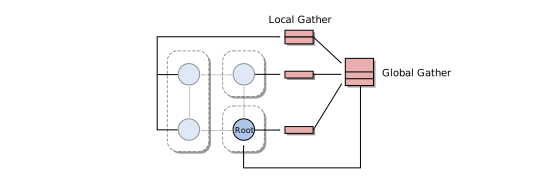
\includegraphics[width=\textwidth]{graphics/30_gvon_collective}
  \caption{Gather operation of the GVON. Data is first locally 
    and then globally collected. Finally, the collected data
    is transmitted to the root vertex.}
  \label{fig:gvon_collective}
\end{figure}


%%%%%%%%%%%%%%%%%%%%%%%%%%%%%%%%%%%%%%%%%%%%%%%%%%%%%%%%%%%%%%%%%%%%%%%%%%%%%%%%
%                                                                              %
% REMAPPING                                                                    %
%                                                                              %
%%%%%%%%%%%%%%%%%%%%%%%%%%%%%%%%%%%%%%%%%%%%%%%%%%%%%%%%%%%%%%%%%%%%%%%%%%%%%%%%
% Checked
\subsection{Remapping of Vertices}
\label{sec:remapping}
Since, the communication topology is separated from the communication
library, it is possible to change the mapping from vertices to peers
at run-time. This run-time behavior is an interesting fact with respect to
load balancing and fault tolerance.

%A remapping repeats the phases distribution and announcement.

Figure~\ref{fig:gvon_remapping} shows the remapping of
vertices of Figure~\ref{fig:gvon_mapping}. The mapping is modified, so that the
vertices are distributed only to two peers. One peer hosts three
vertices and the other one vertex. The third peer is no host of this
graph anymore.

\begin{figure}[H]
  \centering
  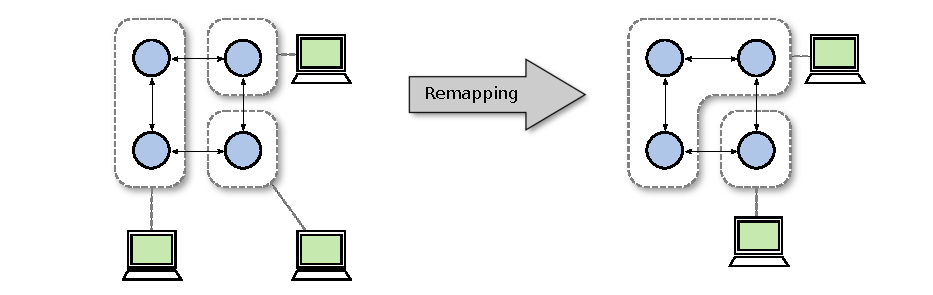
\includegraphics[width=\textwidth]{graphics/30_gvon_remapping}
  \caption{Redistribution of vertices to peers. The number of host of
    the graph is reduced from three hosts to two hosts.}
  \label{fig:gvon_remapping}
\end{figure}

Load balancing can be an issue when the communication topology is
changing during simulation execution. For example could the GoL
simulation add a new rule, which leads to a changed communication
topology for that in turn exists a better vertex mapping.  Even if the
performance of a network link drops, so that some peers are not able
to reach accetable latency and bandwidth among each other, a
remapping could solve this problem at run-time.

A traditional field of application for remapping would be unbalanced
workload in the simulation application. The workload could be
monitored and in unbalanced could a remapping rearrange the workload
in a fair way.

Another issue is the failure of single cluster nodes and therefore
also a failure of hosts located on this nodes. Assuming, that the data
of hosts where check pointed, the hosted vertices of the failed host
can be adopted by another host, also at run-time.

The process of remapping is very similar to the mapping process of
Section~\ref{sec:mapping}.  It is also divided in two phases:
distribution and announcment. It has to be distinguished between
global and local remapping. A global remapping is a repetition of the
mapping process of Section~\ref{sec:mapping}.  Since, local remapping
situation is slightly different, because the hosts already own a set
of hosted vertices, it does not require a redistribution of all
vertices.  The distribution is more a swap or occupation of vertices.

\cleardoublepage

%%% Local Variables:
%%% TeX-master: "diplom"
%%% End:
